\documentclass{article}
\usepackage[utf8]{inputenc}
\usepackage[T1]{fontenc}
\usepackage{graphicx}
\usepackage{hyperref}
\usepackage{geometry}
\geometry{margin=1in}

\title{O P T I C S 427}
\date{Encyclopaedia Britannica (1771)}

\begin{document}
\maketitle

\section*{Historical source}
\textbf{Entry ID:} \texttt{entry-o-p-t-i-c-s-427-681} \\
\textbf{Volume ID:} 144850368 \\
\textbf{Character Count:} 10857

\subsection*{Extracted Text}
the eye at a: fo that none of the rays that fall above \_h\_ on below i, can be reflected to the eye at o; and the dif. stance between \_6 and i is equal to half the length of the object \_AB.\_

Hence it appears, that if a man fees like whole image in a plane looking glats, the part of the glats that reflects his image melt be jull half as long and half as broad as himself, let him fland at any distance from it whatever; and that this image mull appear just as far behind the glafs as he is before it. Thus, the man AB (No. 30.) viewing himself in the plane mirrored CD, which is jull half as long as himself, fees his whole image as at \_EF\_, behind the glafs exactly equal to his own fzz. For, a ray AC, proceeding from his eye at A, and falling perpendicularly upon the surface of the glafs at G, is re-flected back to his eye, in the frame line CaI : and the eye of this image will appear at B, in the frame line pro-duced to E, beyond the glafs. And a ray BD, wrong from his foot, and falling obliquely on the glafs at D, will be reflected as obliquely on the other side of the perpendicular AD), in the direction D,K, and the foot of this image will appear at Ft, in the direction of the re-fled ray AD, produced to F, where is is cut by the right line ACE, drawn parallel to the right line ACE. Jull the fans as if the glafs were taken away, and a real man flood at F, equal in five to the man (handing as B: for to his eyes at A, the eye of the other man at E would be few in the direction of the line ACE; and the foot of the man as F would be seen by the eye A, in the direrection of the line ADF.

\_Of the\_ MAGIC LANTERN.

ABCD (No. 31.) is a tin lantern, with a tube nklm fixed in the field of it. This tube conflicts of two joints, one of which dips into the others and by drawing this joint out, or pulling it in, the tube may be made longer or shorter. At kl in the end of the moveable joint of the tube, a convex lens is fixed, and an object painted with transparent colors upon a piece of thin glafs is pla- edat de homewhere in the immovable joint of the tube; fo that as the tube is lengthened or fluorescent, the lens will be either at a greater or a left distance from this transferen object. In the field of the lantern three is a very convex lens bbc, which ferries to call a very frong light from the candle within the lantern upon the object de. New when the rays, which fringe through the objet de, diverge from the several points as Å, a, sc. in the object, and fall upon the lens kl, they will be made to converge to as many points fj, g \&e. on the other ride of the lens, and will point an inverted picture of the

**Vox. III. No §7.**

object at fg upon a white wall, a fiecet or a fireen of white paper, provided the object is farther from the less than its principal focus. To make this picture appear, dificent and brighty, it must have no other light fall up- on it but what comes through the lens kl ; and for this reason the whole apparatus is to be placed in a dark, room EFGH. The lens A mull be very convex, fo that the object de may be very near to it, and yet not be near- orthan its principal focus; for by this means, as the object is near to the lens, the picture fg will be at a great distance from it , and consequently the picture will be much bigger than the object. Since the picture is inverted in respect of the object, in order to make the picture appear with the right end upwards, it is neceflary that the object de should be placed with the wrong end upwards.

\_Of the\_ DIFFERENT REFRANGIBILITY of LIGHT.

We have hitherto toppofed that a particle of light, as it comes from the fun, is the leaf particular iron which light can be separated. But we mull now correct this top-polition, by thawing, that a particle of light, as it comes from the fun, is, properly speaking, a bundle of rays, which may be farated from one another. Therefore, for the future, by a ray of light we mull be understood to mean, not that collection of particles which we have hitherto called by this name, but the leaf particles in- to which light can be farated.

\_Rays of light are laid to be differently refrangible, when an the form or equal angles of incidence forms are more turned out of the way than others.\_

\_Rays are laid to be differently refasible, if firms are more safely reflected than others.\_

\_Light is called homogeneous, when all the rays are e- quality refrangible: i is treated heterogeneous, when time rays are other refrangible than others.\_

\_The colours of homogeneous light are called primary or female colours ; and thief of heterogeneous light are called secondary or mixed.\_

\_The rays of the fun are not all equally refrangible: and thief rays, which have a different degree of re-fragibility, here likewise a different colors.\_

If a beam of light SF, (No. 32.) that comes from the fun, paths into a dark room through F a round hole in a window fluter EG ; this beam proceeding straight forwards, and falling upon a paper as Y, would there make a round picture of the fun. This picture would be a confufed one indeed, if the hole is a large one and there is no lens in the hole. However, as this round f spotlight a a picture of the fun, we shall hereafter, notwithflanking its condition, call it by this name. Now it a glafs prifm ABC is placed between the hole in the window-fluiter and the paper at Y, the rays of this term; by the refraction which they differ in the prifm, will be bent from their fruit courte, and instead of going to io as to fall upon the paper at Y, they will be turned upwards, and the picture of the fun produced by them will fall up- on a paper MN that is placed above Y. If all the rays **OYI ( 447)** **OUS** 1. Aries, or ram and fleep, the horos of which are flu- ped like a half moon, and compreffed. This animal is perhaps the molt gentle and notifintive, and at the fame time the molt timid and fliquid, of all quadrupeds. In a flock of fleep, there is always a leader, whole flesh the cell amplified and blindly follow. If the men over a precipice, the whole flock follow his example, and cannot be reiftained though evident defiruation be the confe- engence. The finalist buffs, if uncommon, makes them run precipitantly against each other, without knowing the cause of their danger, or belogable to extricate them, folves. In favor, they remain fixed in the fate fots and continue disbursing in this situation, under they are forced to move by the flhepherd or his dog. But through daftally in itself, though altro devoid of feminine and mental qualities, this animal is of the molt extective uitality to man. It infacts on both the and climbing, fer- files the advantages we derive from its milk, its flow, and its rollow.

Love, the lifeliftentment in all animals, is the on- ly pathion which infiples the ram with any degree of vi- vacity; when under the influence of this pallon, he bo- come prettien, more significant and sometimes even attacks the flhepherh himself. But the ew, so fit- male, though in the fame litution, does not appear to be in the last affected; it the items to have no other difficult than that of simply admitting the embraces of the ram, eating her food, and recognizing her offspring; the lamb, on the other hand, is endowed with the fame inflint of diliguishing its means from the self of the dock.

This animal, fo fo and lo simple in its nature and disposition, is likewise extremely weak and feeble in its condition: They can endere but little fingers when ever they ran, their hearts pute, and their wind falls there, they are equally incapable of clearing her or cold, fawor or rain: They are fuject to many difades, molt of which the consensus: They bring forth their young with pain and difficulty, and require more care and attention than any other scientific animal.

The rains capable of generations at the aged 18 months; and the cow carbe impregnated when a year old. One ram is sufficient for go or upo even. He ought to be flrog, well proportioned; his head should be thick and floreg, his front large, his eyes block, his mole fits, his neck thick, his body long and tall, has articles muffy, and his tail long. White is the belt colour for a ram. The ew whose wool is molt plentiful, bulhy, long, fot, and white, the most proper for breeders. Especially when at the fame time they are of a large size, have a thick neck, and move rimbly.

cancer, in azobby. See Leo.

Ewes are generally in fields from the mof of the obber to the beginning of April. However, they may be impeg- nated as any time, it they be fed with illuminating non- rilmen, as fat water, and bread made of hem-feed. They go with your about, few months, and generally bring forth, but one at a time, though frequently two. In warm climates, they may bring forth twice in a year, but in Britain, France, and molt parts of Europe, only enough. They goes milk plentyfully for tenx or eight minutes: Their milk affords mouthments for children broad country people; good checefe is made of it, especially women mixed with cow-milk. They live from 10 to 12 thyvers, and are capable of bringing forth an long as they tailites.

When the mile limbs are not intended to be keys for propagation, but farmed for food, they might to be calibrated at the age of five or fix months. This operation is performed two ways: in the one, an inclion is made and the facilities taken on; in the other, a liature is tied by around the forearm, above the facilities, which foot deftroys the veffels which nourish them. After ca- affirates, they are called wearless.

The new, ewes, and weather, when one year old, lofs the two foreseeh of the under jaw; fix months after- wards, they lofe the two foreseeh next to thele; and at the age of three years, the teeth are all replaced. The age of a ram may likewise be delivered by their home, which always appears the left year, and frequently saboon as they are brought forth. Their horse uniformly ac- quite an additional ring every year as longer the creature lives. The ews commonly have an horses, but a kind of long protubrances in place of them: However, fome of them have two, and some four hors.

In Spain, and the Southern passa of Europe, the flocks are kept in thudes or fiables during the night; but in Britain, where there is now no danger from wolves, they are allowed to remain without; both adult and day; which make the animals more healthy, and their dish a more whole food. Dry and mountainous grounds, where thyme and fleep's fefea grafs abound, are the built for the patturing fleep.

2. The Guinemands, or Guinea fleep, has pendulous ears, lax hairy dew lips, and a prominence on the hind part of the head. The weol is short, like that of a goat. It is a native of Guinea.

3. The fireplaces, or Cretan fleep, has fruit ceri- nated horses, twilled in a firal manner. It is a native of Mount folia.



\section*{Source record}
\begin{itemize}
\item \textbf{Dataset:} \texttt{NationalLibraryOfScotland/encyclopaedia\_britannica\_illustrated}
\item \textbf{Dataset Revision:} \texttt{309f765b1ecc83e0a7f7762e44b4a927a7555443}
\item \textbf{Page ID:} \texttt{britannica:309f765b1ecc83e0a7f7762e44b4a927a7555443:train:681} \\
  \textbf{Filename:} \texttt{page-0681-c2be06f2d615.jpg} \\
  \textbf{Row Index:} 681 \\
  \textbf{SHA256:} \texttt{c2be06f2d6151658...}
\item \textbf{Page ID:} \texttt{britannica:309f765b1ecc83e0a7f7762e44b4a927a7555443:train:713} \\
  \textbf{Filename:} \texttt{page-0713-3db0c66f81f4.jpg} \\
  \textbf{Row Index:} 713 \\
  \textbf{SHA256:} \texttt{3db0c66f81f48bd0...}
\end{itemize}

\begin{figure}[h]
\centering
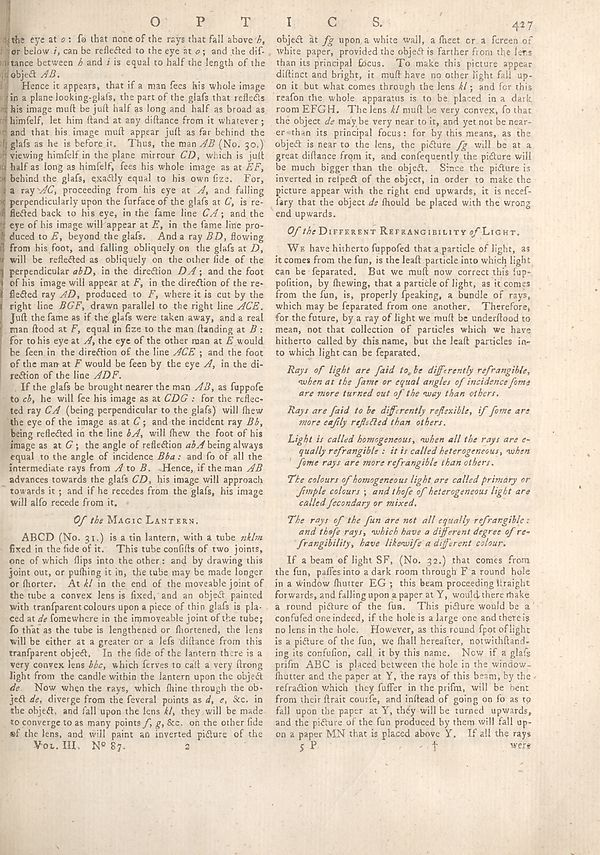
\includegraphics[width=0.85\textwidth]{../scans/page-0681-c2be06f2d615.jpg}
\caption*{Source scan: \texttt{page-0681-c2be06f2d615.jpg}}
\end{figure}
\begin{figure}[h]
\centering
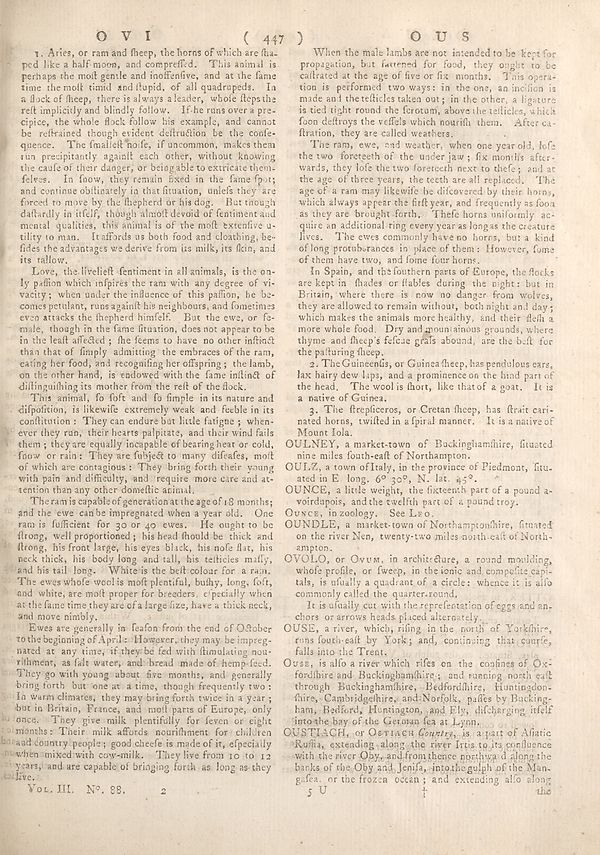
\includegraphics[width=0.85\textwidth]{../scans/page-0713-3db0c66f81f4.jpg}
\caption*{Source scan: \texttt{page-0713-3db0c66f81f4.jpg}}
\end{figure}

\end{document}
